% !TeX program = lualatex
% ==================================================================
%  卒業論文（たたき台）
%  RNN を用いたニューロンモデルの代理モデル構築
%
%  コンパイル: lualatex 卒業論文.tex を2回
%             （目次・相互参照のため2回必要。latexmk 卒業論文.tex でもよい）
%
%  【このファイルの使い方】
%  ・\TODO{...} は「これから書く／確かめる」箇所。本文中に赤字で表示される。
%    提出前に \TODO を全部消すこと（\listoftodo は使っていないので grep で探す）。
%  ・すでに確定している内容（HHモデルの式、RNNの式、BPTTの式、
%    sin波での動作確認）は本文として書き込んである。
%  ・構成は棟近先輩の卒業論文（SINDy版）の章立てを踏襲しているが、
%    手法が SINDy → RNN に変わる部分は差し替えてある。
% ==================================================================
\documentclass[a4paper,11pt,openany]{ltjsreport}

\usepackage{amsmath,amssymb,mathtools}
\usepackage{bm}
\usepackage{siunitx}
\usepackage{graphicx}
\usepackage{booktabs}
\usepackage{array}
\usepackage{multirow}
\usepackage{enumitem}
\usepackage{algorithm}
\usepackage{algpseudocode}
\usepackage{xcolor}
\usepackage[hidelinks]{hyperref}
\usepackage{geometry}
\geometry{a4paper,top=30mm,bottom=30mm,left=25mm,right=25mm}

% --- 書きかけの箇所を目立たせるコマンド（提出前に中身を消す）---
\newcommand{\TODO}[1]{\textcolor{red}{\textbf{[TODO: #1]}}}

% --- よく使う記号のマクロ ---
\newcommand{\Iext}{I_{\mathrm{ext}}}
\newcommand{\gleak}{g_{\mathrm{leak}}}
\newcommand{\gNa}{g_{\mathrm{Na}}}
\newcommand{\gK}{g_{\mathrm{K}}}
\newcommand{\ENa}{E_{\mathrm{Na}}}
\newcommand{\EK}{E_{\mathrm{K}}}
\newcommand{\Eleak}{E_{\mathrm{leak}}}
\newcommand{\Ileak}{I_{\mathrm{leak}}}
\newcommand{\INa}{I_{\mathrm{Na}}}
\newcommand{\IK}{I_{\mathrm{K}}}

\algrenewcommand\algorithmicrequire{\textbf{Require:}}
\algrenewcommand\algorithmicensure{\textbf{Ensure:}}

\title{リカレントニューラルネットワークを用いた\\ニューロンモデルの代理モデルの構築}
\author{山下 陽平}
\date{令和 8 年度}

\begin{document}

% ==================================================================
% 表紙
% ==================================================================
\begin{titlepage}
  \centering
  \vspace*{20mm}
  {\Large 令和 8 年度}\\[15mm]
  {\LARGE 卒業論文}\\[25mm]
  {\LARGE リカレントニューラルネットワークを用いた}\\[3mm]
  {\LARGE ニューロンモデルの代理モデルの構築}\\[35mm]
  % \TODO{題目は仮。Multi-Compartment まで到達できるかで変わるため、
  %       最終的な結果が出てから確定させる}
  {\large 指導教員 小林 泰良 助教}\\[20mm]
  {\large 山口大学}\\[3mm]
  {\large 理学部\quad 物理・情報科学科}\\[3mm]
  {\large 情報科学コース 4年}\\[20mm]
  {\large 山下 陽平}
  \vfill
\end{titlepage}

\tableofcontents
\clearpage

% ==================================================================
\chapter{はじめに}
% ==================================================================

脳は生物の思考や行動といった情報処理を司る器官であり、その機能はニューロンの
ネットワーク上を伝播するスパイクによって実現される\cite{yamazaki2021}。
脳の情報処理の仕組みを知るためにはネットワーク上のスパイクを観測する必要があるが、
実際の脳は莫大な数（$10^{11}$ 個程度\cite{kandel2022}）のニューロンから構成されるため、
そのすべてを同時に観測することは極めて難しい。一方で、個別のニューロンの振る舞いに
ついては多くのことが知られている。そのため、ニューロンの振る舞いを記述する数理モデルを
組み合わせた脳モデルを構築し、計算機上でシミュレーションを行うという手法が広く
用いられている。

近年の研究によると、ニューロンは刺激シーケンスの弁別や排他的論理和演算といった
複雑な演算を行っており、これにはニューロンそのものが持つ空間形状が大きく関わっている
ことが分かってきた\cite{gidon2020,branco2010}。
ニューロンの空間形状をモデル化に組み入れた数理モデルが Multi-Compartment モデルであり、
このモデルはニューロンを電気的に連結された複数の区画（コンパートメント）の群として
表現することで、上記のような特性を忠実に再現する。
しかし、Multi-Compartment モデルは各コンパートメントが膜電位と複数の隠れ変数を
状態として保持するため、シミュレーションに多くのメモリを必要とする\cite{yamazaki2021}。
マウスの脳（約 $10^{8\sim9}$ 個のニューロンを持つ）程度の規模であっても、
国内最高性能のスーパーコンピュータである富岳でも扱いきれないほどに
空間計算量が増大してしまう\cite{kobayashi2024}。
脳シミュレーションにおいては、隠れ変数の値そのものを直接知る必要はないにもかかわらず、
隠れ変数を格納するためのメモリはニューロン数とコンパートメント数に比例して
増加してしまう。したがって、大規模な脳モデルのシミュレーションを実現するためには、
ニューロンモデルをシミュレーションする際の計算コストを削減することが重要である。

計算コストを削減する手法として、本研究では代理モデル（surrogate model）の構築を考える。
ここでの代理モデルとは、元のニューロンモデルに対し、より少ない隠れ変数、
あるいはより高速な計算で同等の膜電位応答を再現できるモデルを指す。
棟近先輩による先行研究では、時系列データから支配方程式をスパースに同定する手法である
SINDy\cite{brunton2015} と主成分分析を組み合わせることで、
Hodgkin-Huxley モデル\cite{hodgkin1952}の 4 つの状態変数
$(V, m, h, n)$ を 2 つ $(V, g')$ に圧縮した代理モデルが構築されている\cite{munechika2025}。
この手法では空間計算量の削減には成功したが、同定された微分方程式の右辺の項数が
十分にスパースにならず、時間計算量はかえって増加するという課題が残されている。

そこで本研究では、代理モデルの構築手法としてリカレントニューラルネットワーク
（Recurrent Neural Network, 以下 RNN）を用いる。RNN を用いる理由は次の 3 点である。

\begin{enumerate}[label=(\arabic*)]
  \item \textbf{内部状態を保持できる}。
        ニューロンモデルにおける現在の膜電位は、現在の入力だけでなく過去の膜電位や
        状態変数にも依存する。RNN は隠れ状態として過去の情報を保持するため、
        このような動的システムの状態遷移を自然に表現できる。
  \item \textbf{時系列データとの親和性が高い}。
        膜電位は時間とともに変化する時系列データであり、RNN は時系列データの
        時間相関を学習するために設計されたモデルである。
  \item \textbf{GPU による高速化が期待できる}。
        RNN の推論は主に行列積で構成されるため、GPU による並列化と相性がよい。
        微分方程式を逐次的に数値積分する従来手法に対し、高速な推論が期待できる。
\end{enumerate}

本研究の最終的な目標は Multi-Compartment モデルに対する代理モデルの構築であるが、
Multi-Compartment モデルは空間形状を考慮した複雑なモデルであるため、
いきなりこれを対象とするのは難易度が高い。そこで、より基本的なニューロンモデルで
RNN による代理モデルが機能するかをまず確かめる。そのようなモデルとして、
空間形状を考慮しないが Multi-Compartment モデルと同様にイオン輸送を制御する
隠れ変数を持つ Hodgkin-Huxley モデルを選ぶ\cite{hodgkin1952}。

また本研究では、RNN の内部で行われる計算を理解することを重視し、
PyTorch などの深層学習フレームワークを用いず、NumPy の基本的な配列演算のみで
RNN を実装する。これにより、順伝播・誤差逆伝播・パラメータ更新の各過程を
すべて追跡可能な形で記述する。

% ==================================================================
\chapter{基礎知識}
% ==================================================================

\section{ニューロンのモデル化}

脳は感覚情報の処理、記憶、思考、運動司令などを司る情報処理器官であり、
これはニューロンのネットワークによって実現される。
ニューロンは電流の入力を受けると、細胞の内外の電位差である膜電位を変化させる。
膜電位の変化には、細胞膜と、細胞膜に埋め込まれたイオンチャネル
（特定のイオンのみを選択的に透過させる輸送体）が深く関わっている。

ニューロンの電気的な振る舞いは、細胞膜を容量 $C$ [\si{\micro F/cm^2}] のキャパシタ、
膜を透過するイオンの流れ $\Ileak$ [\si{\micro A/cm^2}] を内部コンダクタンス
$\gleak$ [\si{mS/cm^2}]、起電力 $E_{\mathrm{eq}}$ [\si{mV}] の電池を流れる電流と
見立てることで、RC 回路とみなすことができる\cite{miyagawa2013}。
外部から入力される電流を $\Iext$ [\si{\micro A/cm^2}] とすると、
膜電位 $V$ の時間変化は次の微分方程式に従う。

\begin{equation}
  C \frac{dV}{dt} = -\gleak\left(V(t) - E_{\mathrm{eq}}\right) + \Iext(t)
  \label{eq:rc}
\end{equation}

このモデルは細胞膜の基本的なダイナミクスを記述しているが、
これだけでは膜電位が上下するのみでスパイクは発射されない。
イオンチャネルの種類まで考慮してモデル化することで、スパイクの発射を再現できる。

\TODO{図 2.1 として RC 回路図を入れる。TikZ で描くか、先輩の卒論の図を参考に自作する}

\section{Hodgkin-Huxley モデル}
\label{sec:hh}

単一ニューロンの数理モデルの中で世界で最初に開発されたものが
Hodgkin-Huxley モデル（以下 HH モデル）である\cite{hodgkin1952}。
HH モデルは、イオン電流をナトリウムイオン電流 $\INa$、カリウムイオン電流 $\IK$、
リーク電流 $\Ileak$（その他のイオン電流）に分離したモデルである。
式\eqref{eq:rc}のイオン電流の項を分割することで、膜電位 $V$ [\si{mV}] の
変化式は次のように書ける。

\begin{equation}
  C\frac{dV}{dt} = -\gleak\left(V(t)-\Eleak\right)
                   -\gNa(V,t)\left(V(t)-\ENa\right)
                   -\gK(V,t)\left(V(t)-\EK\right) + \Iext(t)
  \label{eq:hh_v}
\end{equation}

ここで、ナトリウムコンダクタンス $\gNa(V,t)$ とカリウムコンダクタンス $\gK(V,t)$ は
$V, t$ に従って変化する。

\begin{align}
  \gNa(V,t) &= \bar{g}_{\mathrm{Na}}\, m^3(V,t)\, h(V,t) \label{eq:gna}\\
  \gK(V,t)  &= \bar{g}_{\mathrm{K}}\, n^4(V,t)           \label{eq:gk}
\end{align}

$\bar{g}_{\mathrm{Na}}, \bar{g}_{\mathrm{K}}$ は各チャネルのコンダクタンスが
とりうる最大値を表す定数（表\ref{tab:hh_const}）であり、
$m, h, n$ は膜電位に依存して変化するゲート変数である。
ゲート変数はイオンチャネルの開口率を表す $0 \sim 1$ の値をとる変数であり、
膜電位と同様に時間に関する一階の微分方程式に従う。

\begin{equation}
  \frac{d}{dt}x(V,t) = \alpha_x(V)\left(1 - x(V,t)\right) - \beta_x(V)\, x(V,t)
  \qquad (x = m, h, n)
  \label{eq:hh_gate}
\end{equation}

$\alpha_x(V), \beta_x(V)$ はそれぞれ次式で定義される。

\begin{align}
  \alpha_m(V) &= \frac{0.1\,(V + 40)}{1 - \exp\left(-\dfrac{V + 40}{10}\right)}, &
  \beta_m(V)  &= 4\exp\left(-\frac{V + 65}{18}\right) \notag\\
  \alpha_h(V) &= 0.07\exp\left(-\frac{V + 65}{20}\right), &
  \beta_h(V)  &= \frac{1}{1 + \exp\left(-\dfrac{V + 35}{10}\right)} \label{eq:rate}\\
  \alpha_n(V) &= \frac{0.01\,(V + 55)}{1 - \exp\left(-\dfrac{V + 55}{10}\right)}, &
  \beta_n(V)  &= 0.125\exp\left(-\frac{V + 65}{80}\right) \notag
\end{align}

ここで、本研究では膜電位 $V$ を、静止膜電位を $-65$ [\si{mV}] とする表記で表している。
Hodgkin と Huxley の原論文\cite{hodgkin1952}および先行研究\cite{munechika2025}では、
静止膜電位を $0$ [\si{mV}] とし脱分極を正の向きにとる表記が用いられているため、
レート関数や反転電位の値の表れ方が異なる。両者は $V$ の原点の取り方が異なるだけで
等価なモデルであるが、本研究では実装に合わせて前者の表記を用いる。

なお、$\alpha_m(V)$ は $V = -40$ [\si{mV}]、$\alpha_n(V)$ は $V = -55$ [\si{mV}] に
おいて分母と分子がともに $0$ となる。実装ではこれらの近傍において、
L'H\^{o}pital の定理から得られる極限値（それぞれ $1.0$ と $0.1$）を用いている。

まとめると、HH モデルは膜電位 $V$ とゲート変数 $m, h, n$ に関する
4 元の連立常微分方程式である。

\begin{table}[htbp]
  \centering
  \caption{Hodgkin-Huxley モデルで使うイオンチャネルに関する定数。
           膜容量は $C = 1.0$ [\si{\micro F/cm^2}] とした。}
  \label{tab:hh_const}
  \begin{tabular}{lrr}
    \toprule
    イオン種 & 反転電位 $E$ [\si{mV}] & 最大コンダクタンス $\bar{g}$ [\si{mS/cm^2}] \\
    \midrule
    $\mathrm{Na}^{+}$      &   50.000 & 120.0 \\
    $\mathrm{K}^{+}$       &  -77.000 &  36.0 \\
    その他のイオン (leak)   &  -54.387 &   0.3 \\
    \bottomrule
  \end{tabular}
\end{table}

\begin{figure}[htbp]
  \centering
  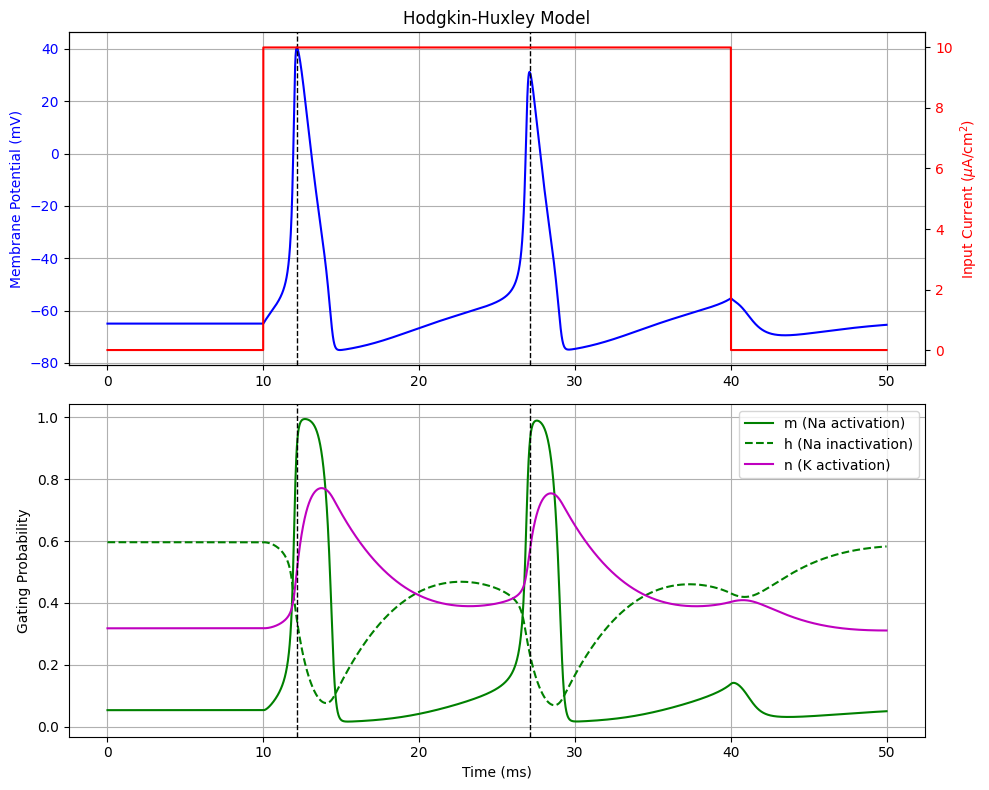
\includegraphics[width=0.85\linewidth]{images/hodgkin_huxley_simulation.png}
  \caption{Hodgkin-Huxley モデルのシミュレーション結果。
           \TODO{図の説明を書く。与えた電流の振幅・時間、上から何のグラフかを明記する}}
  \label{fig:hh_sim}
\end{figure}

\section{Multi-Compartment モデル}

Multi-Compartment モデルは、ニューロンの空間形状を電気的に連結された
複数のコンパートメントとして表現したニューロンモデルである。
各コンパートメントはそれぞれ膜電位と状態変数を持ち、
隣接するコンパートメントとの間には電位差に比例した軸方向電流が流れる。
コンパートメント $i$ に流れ込む軸方向電流は次式で表される。

\begin{equation}
  I_i^{(\mathrm{axial})} = \sum_{j \in \mathrm{neighbors}} g_{i,j}\left(V_j - V_i\right) + I_{\mathrm{inj}}
  \label{eq:axial}
\end{equation}

\TODO{どの Multi-Compartment モデルを対象とするかが決まっていない。
      小林先生から紹介された論文を読んで、対象とするモデル（コンパートメント数、
      各コンパートメントの種類）を確定させ、ここに記述する}

\TODO{HH コンパートメントと Passive コンパートメントの区別について書く。
      HH コンパートメントは $I_{\mathrm{ion}}$ がスパイクの発射を駆動し、
      Passive コンパートメントは $C_m dV/dt = -g_{\mathrm{leak}}(V-E_{\mathrm{rest}}) + \Iext$
      のみで受動的に振る舞う}

\section{リカレントニューラルネットワーク}

\subsection{時系列データと過去の隠れ層}

RNN は、並びに規則性のあるデータを学習することで、
未知の時系列データが与えられたときにその未来の状態を予測するモデルである。
時系列データを扱うためには、過去の状態をモデル内に保持し、
現在に対する過去からの影響を把握しておく必要がある。
一般的なニューラルネットワークは「入力層 $\bm{x}(t)$ -- 隠れ層 $\bm{h}(t)$ --
出力層 $\bm{y}(t)$」という構造を持つが、
RNN ではこれに加えて時刻 $t-1$ における隠れ層の値 $\bm{h}(t-1)$ を保持しておき、
それも時刻 $t$ の隠れ層に伝える\cite{sugomori2019}。
時刻 $t$ の状態を $t-1$ の状態として保持しフィードバックさせるため、
$\bm{h}(t-1)$ には再帰的に過去の状態がすべて反映されていることになる。
これがリカレント（再帰型）ニューラルネットワークと呼ばれる理由である。

\begin{figure}[htbp]
  \centering
  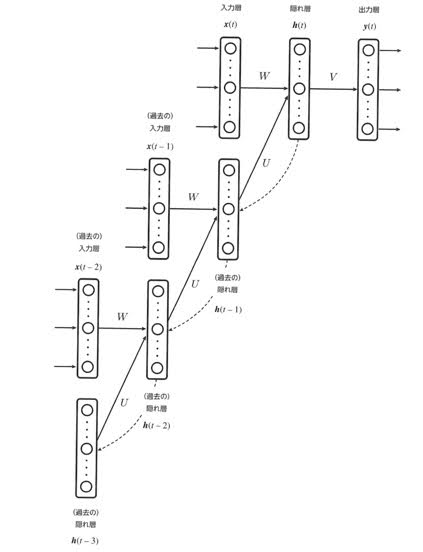
\includegraphics[width=0.6\linewidth]{images/rnn_hidden_state_diagram.png}
  \caption{過去の隠れ層を加えたニューラルネットワークの構造。}
  \label{fig:rnn_diagram}
\end{figure}

\subsection{モデル化}

最も基本的な RNN（Elman 型\cite{elman1990}）では、隠れ層と出力層は次式で表される。

\begin{align}
  \bm{h}(t) &= f\left(W\bm{x}(t) + U\bm{h}(t-1) + \bm{b}\right) \label{eq:rnn_h}\\
  \bm{y}(t) &= g\left(V\bm{h}(t) + \bm{c}\right)                \label{eq:rnn_y}
\end{align}

ここで $f(\cdot), g(\cdot)$ は活性化関数、$\bm{b}, \bm{c}$ はバイアスベクトルである。
$W$ は入力層から隠れ層への重み、$U$ は過去の隠れ層から隠れ層への重み（再帰重み）、
$V$ は隠れ層から出力層への重みを表す。
隠れ層の式に過去から順伝播してくる項 $U\bm{h}(t-1)$ が付くが、
それ以外は一般的なニューラルネットワークと違いはない。
そのため、各パラメータも誤差逆伝播法により最適化できる。

再帰計算を含む場合、活性化関数 $f$ には注意が必要である。
通常のニューラルネットワークでは ReLU が効果的であるが、
ReLU は出力が入力に比例し最大値が $+\infty$ であるため、
同じ重みが繰り返し掛けられる再帰計算ではオーバーフローを起こす可能性がある。
そのため、出力値が一定範囲に収まる双曲線正接関数 $\tanh$ が用いられるのが
一般的である\cite{sugomori2019}。本研究でも $f = \tanh$ とする。

\subsection{Backpropagation Through Time}

誤差関数を $E$ とし、隠れ層・出力層の活性化前の値をそれぞれ

\begin{align}
  \bm{p}(t) &\coloneqq W\bm{x}(t) + U\bm{h}(t-1) + \bm{b} \label{eq:p}\\
  \bm{q}(t) &\coloneqq V\bm{h}(t) + \bm{c}                \label{eq:q}
\end{align}

と定義する。これに対する誤差項を

\begin{equation}
  \bm{e}_h(t) \coloneqq \frac{\partial E}{\partial \bm{p}(t)}, \qquad
  \bm{e}_o(t) \coloneqq \frac{\partial E}{\partial \bm{q}(t)}
  \label{eq:err}
\end{equation}

とすると、各パラメータの勾配は次のように表せる。

\begin{align}
  \frac{\partial E}{\partial W} &= \bm{e}_h(t)\,\bm{x}(t)^{\mathsf{T}} &
  \frac{\partial E}{\partial \bm{b}} &= \bm{e}_h(t) \notag\\
  \frac{\partial E}{\partial U} &= \bm{e}_h(t)\,\bm{h}(t-1)^{\mathsf{T}} &
  \frac{\partial E}{\partial \bm{c}} &= \bm{e}_o(t) \label{eq:grads}\\
  \frac{\partial E}{\partial V} &= \bm{e}_o(t)\,\bm{h}(t)^{\mathsf{T}} & & \notag
\end{align}

ここで注意すべき点がある。一般的なニューラルネットワークでは、
誤差関数を 2 乗誤差関数とする場合、誤差項は

\begin{align}
  \bm{e}_h(t) &= f'(\bm{p}(t)) \odot V^{\mathsf{T}}\bm{e}_o(t) \label{eq:eh}\\
  \bm{e}_o(t) &= g'(\bm{q}(t)) \odot \left(\bm{y}(t) - \bm{t}(t)\right) \label{eq:eo}
\end{align}

で与えられる。これらの式自体は正しいが、RNN ではネットワークの順伝播で
時刻 $t-1$ における隠れ層の出力 $\bm{h}(t-1)$ を考えたため、
逆伝播の際も $t-1$ における誤差を考える必要がある。
すなわち、順伝播において $\bm{h}(t)$ が $\bm{h}(t-1)$ の再帰関係式で
表されたのと同様に、逆伝播では $\bm{e}_h(t-1)$ を $\bm{e}_h(t)$ の式で
表す必要がある。このとき誤差は時間を遡って逆伝播していることになるので、
これを Backpropagation Through Time（以下 BPTT）と呼ぶ\cite{werbos1990}。

$\bm{e}_h(t-1) = \partial E / \partial \bm{p}(t-1)$ であることから、
再帰関係式を求めると

\begin{align}
  \bm{e}_h(t-1)
   &= \frac{\partial E}{\partial \bm{p}(t)} \odot \frac{\partial \bm{p}(t)}{\partial \bm{p}(t-1)} \notag\\
   &= \bm{e}_h(t) \odot \left(
        \frac{\partial \bm{p}(t)}{\partial \bm{h}(t-1)}
        \frac{\partial \bm{h}(t-1)}{\partial \bm{p}(t-1)} \right) \label{eq:bptt}\\
   &= \bm{e}_h(t) \odot \left( U f'(\bm{p}(t-1)) \right) \notag
\end{align}

が得られる。よって、再帰的に

\begin{equation}
  \bm{e}_h(t-z-1) = \bm{e}_h(t-z) \odot \left( U f'(\bm{p}(t-z-1)) \right)
  \label{eq:bptt_z}
\end{equation}

の関係で表すことができる。これによりすべての勾配が計算できるため、
各パラメータの更新式は学習率を $\eta$ として次のようになる。

\begin{align}
  W(t+1) &= W(t) - \eta \sum_{z=0}^{\tau} \bm{e}_h(t-z)\,\bm{x}(t-z)^{\mathsf{T}} \notag\\
  U(t+1) &= U(t) - \eta \sum_{z=0}^{\tau} \bm{e}_h(t-z)\,\bm{h}(t-z-1)^{\mathsf{T}} \notag\\
  V(t+1) &= V(t) - \eta\, \bm{e}_o(t)\,\bm{h}(t)^{\mathsf{T}} \label{eq:update}\\
  \bm{b}(t+1) &= \bm{b}(t) - \eta \sum_{z=0}^{\tau} \bm{e}_h(t-z) \notag\\
  \bm{c}(t+1) &= \bm{c}(t) - \eta\, \bm{e}_o(t) \notag
\end{align}

この $\tau$ がどれくらいの過去まで遡って時間依存性を見るか（すなわちデータ長）を
表すので、理想的には $\tau \to +\infty$ とすべきである。
しかし、現実には勾配が消失（あるいは爆発）してしまうことを防ぐため、
$\tau = 10 \sim 100$ 程度に設定するのが一般的である\cite{sugomori2019}。

\subsection{再帰計算がある場合の重みの初期値}

ネットワークの順伝播を考えると、隠れ層の再帰部分には同じ重み $U$ が
繰り返し掛けられることになる。そのため、通常のニューラルネットワークの
初期化手法（Xavier の初期化など）を用いると、計算中にオーバーフローを
起こす可能性が高くなる。

そこで用いられるのが直交行列による初期化である\cite{saxe2014}。
直交行列とは、正方行列 $U$ に対して $UU^{\mathsf{T}} = I$、
すなわち $U^{-1} = U^{\mathsf{T}}$ となる行列を指す。
重みが直交行列として初期化されていれば、再帰計算を行っても
オーバーフローを起こしにくくなるため、計算の安定化が見込める。

% ==================================================================
\chapter{RNN による代理モデルの構築手法}
% ==================================================================

\section{概要}

本研究では、外部電流 $\Iext(t)$ に対する膜電位 $V(t)$ の応答を、
微分方程式を数値積分する代わりに RNN の推論によって再現する代理モデルを構築する。
具体的な手順は次のとおりである。

\begin{enumerate}
  \item HH モデルのシミュレーションを陽的 Euler 法により行い、
        ランダムな外部入力 $\Iext$ に対する $V(t), m(t), h(t), n(t)$ の
        時系列データを取得する（\ref{sec:sim_cond}節）。
  \item 得られた時系列データを、RNN が学習できる形式（一定長の系列とその直後の値の組）
        に変換する（\ref{sec:dataset}節）。
  \item NumPy のみを用いて実装した RNN に、このデータを学習させる（\ref{sec:rnn_impl}節）。
  \item 学習済みの RNN に外部電流を与え、膜電位応答を逐次的に生成させる
        （\ref{sec:inference}節）。
  \item 生成された膜電位応答を、元の HH モデルの応答と比較して評価する
        （\ref{sec:metrics}節）。
\end{enumerate}

\TODO{RNN に何を入力し何を出力させるかが最大の設計上の論点であり、まだ確定していない。
      現時点で考えている候補を以下に挙げる。実験して決める。\\
      (a) 入力 $\Iext$ の系列 $\to$ 出力 $V$（最も素朴。隠れ変数を完全に隠蔽できる）\\
      (b) 入力 $(\Iext, V)$ の系列 $\to$ 出力 次時刻の $V$（自己回帰。学習は容易だが誤差が累積する）\\
      (c) 入力 $(\Iext, V, m, h, n)$ $\to$ 出力 次時刻の $(V, m, h, n)$（微分方程式の右辺を学習させる形）\\
      (d) 一部を HH モデル、一部を RNN で置き換えるハイブリッド}

\section{シミュレーション条件}
\label{sec:sim_cond}

\subsection{Euler 法}

HH モデルの実体は $n$ 元 1 階連立常微分方程式

\begin{equation}
  \frac{d\bm{x}}{dt} = \bm{f}(\bm{x}, t)
  \label{eq:ode}
\end{equation}

である。今回扱うモデルにおいては $\bm{f}$ が非線形の関数であるため、
解析解を求めることは非常に困難である。そこで、シミュレーションの手法として
数値計算手法の一つである陽的 Euler 法を用いた。
Euler 法では、区間 $[a,b]$ を刻み幅 $h$ で等間隔に $n$ 等分した点
$t_0, t_1, \dots, t_n$ に対し、各点での近似解 $x_0, x_1, \dots, x_n$ を
Algorithm \ref{alg:euler} のように求める\cite{minemura2008}。

\begin{algorithm}[htbp]
  \caption{Euler 法}
  \label{alg:euler}
  \begin{algorithmic}[1]
    \Require 初期値 $c_0$、刻み幅 $h$
    \State $x_0 \gets c_0$
    \For{$i = 0, 1, \dots, n-1$}
      \State $x_{i+1} \gets x_i + h\, f(x_i, t_i)$
    \EndFor
    \State \Return $x_0, x_1, \dots, x_n$
  \end{algorithmic}
\end{algorithm}

\subsection{初期値の与え方}

膜電位の初期値は静止膜電位 $V_{\mathrm{rest}} = -65.0$ [\si{mV}] を与える。
これは\ref{sec:hh}節で述べた表記（静止膜電位を $-65$ [\si{mV}] とする表記）に
対応しており、式\eqref{eq:rate}のレート関数もこの表記のもとで定義されている。

ゲート変数の初期値については、式\eqref{eq:hh_gate}を変形すると

\begin{equation}
  \frac{1}{\alpha_x(V) + \beta_x(V)} \frac{dx}{dt}
    = -\left( x - \frac{\alpha_x(V)}{\alpha_x(V) + \beta_x(V)} \right)
  \label{eq:gate_relax}
\end{equation}

となる。この式は、ゲート変数 $x$ が $\alpha_x(V) / (\alpha_x(V) + \beta_x(V))$ に
おいて $dx/dt = 0$、すなわち定常状態になることを意味する。
時刻 $t=0$ の初期値において傾きが $0$ であってほしいので、
ゲート変数の初期値は

\begin{equation}
  \begin{pmatrix} m_0 \\ h_0 \\ n_0 \end{pmatrix}
  = \begin{pmatrix}
      \alpha_m(V_0) / (\alpha_m(V_0) + \beta_m(V_0)) \\
      \alpha_h(V_0) / (\alpha_h(V_0) + \beta_h(V_0)) \\
      \alpha_n(V_0) / (\alpha_n(V_0) + \beta_n(V_0))
    \end{pmatrix}
  \label{eq:gate_init}
\end{equation}

とする。

\subsection{外部電流の生成方法}

教師データには、なるべく様々な入力とそれに対する応答が含まれることが望ましい。
様々な入力が教師データの中に存在すれば、特定の入力に依存しないロバストなモデルの
構築が期待できる。そこで、教師データに用いる外部電流 $\Iext$ は、
ランダムな振幅を持つパルス電流の組み合わせとして与える
（Algorithm \ref{alg:iext}）。

\begin{algorithm}[htbp]
  \caption{$\Iext$ の決定}
  \label{alg:iext}
  \begin{algorithmic}[1]
    \Require シミュレーション時間 $T_{\mathrm{sim}}$、時間間隔 $\Delta (\ll T_{\mathrm{sim}})$、
             電流の範囲 $[I_{\min}, I_{\max}]$
    \State 区間 $[0, T_{\mathrm{sim}}]$ を $\Delta$ で分割し、
           $t_0 = [0,\Delta], t_1 = [\Delta, 2\Delta], \dots$ を得る
    \For{$i = 0, 1, \dots, n$}
      \State $[I_{\min}, I_{\max}]$ の中から一様乱数で $I_{\mathrm{rnd}}$ を選ぶ
      \State 区間 $t_i$ の間は $I_{\mathrm{rnd}}$ [\si{mA}] の定常電流が流れているものとする
    \EndFor
    \State \Return $\Iext = [\Iext^{(0)}, \Iext^{(1)}, \dots, \Iext^{(n)}]$
  \end{algorithmic}
\end{algorithm}

\TODO{パラメータを確定させる。先行研究\cite{munechika2025}では
      $\Delta = 10$ ms、$I_{\max} = 20$ mA、$dt = 0.05$ ms、$T_{\mathrm{sim}} = 900$ ms、
      最新の進捗報告では $-5 \sim 20$ mA、$20$ ms 幅、$dt = 0.01$ ms が使われている。
      本研究でどの条件を使うかを決め、その理由も書く}

\section{学習データの作成}
\label{sec:dataset}

RNN の学習には、一定長の入力系列とその直後の正解値の組が必要である。
系列長を $\tau$ として、時系列データ $f(0), f(1), \dots$ を次のように分割する。

\begin{equation}
  \left[ f(t),\, f(t+1),\, \dots,\, f(t+\tau-1) \right] \longrightarrow f(t+\tau)
  \label{eq:window}
\end{equation}

すなわち、$\tau$ 点の系列を入力とし、その次の 1 点を予測する教師あり学習とする。
窓を 1 時刻ずつずらしながらこの組を作るため、
元の時系列の長さを $L$ とするとサンプル数は $L - \tau$ となる。
入力データ $X$ と正解データ$\bm{t}$ の形状はそれぞれ

\begin{equation}
  X \in \mathbb{R}^{(L-\tau) \times \tau \times D}, \qquad
  \bm{t} \in \mathbb{R}^{(L-\tau) \times K}
  \label{eq:shapes}
\end{equation}

となる（$D$ は入力次元、$K$ は出力次元）。
一定長に分割するのは BPTT における計算の都合という理由もあるが、
データ数を増やして学習できるという理由もある\cite{sugomori2019}。

得られたデータは訓練データと検証データに分割する。
ただし時系列データを扱う場合、未来の時刻のデータが訓練データに含まれないように
しなければならない。すなわち、全データをランダムにシャッフルするのではなく、
前から順に一定数を訓練データ、残りを検証データとする。
本研究では訓練データ $80\%$、検証データ $20\%$ とした。

\TODO{膜電位は $-65 \sim +40$ mV 程度、ゲート変数は $0 \sim 1$ と
      スケールが大きく異なるため、正規化（標準化）が必要になると思われる。
      どの正規化を行ったかをここに書く}

\section{RNN の実装}
\label{sec:rnn_impl}

本研究では、RNN の内部計算を理解することを目的として、
PyTorch などのフレームワークを使わず NumPy の基本的な配列演算のみで
RNN を実装した。以下、実装した処理を順に述べる。

\subsection{順伝播}

時刻 $t = 0$ には 1 つ前の時刻が存在しないため、隠れ状態の初期値は
$\bm{h}(-1) = \bm{0}$ とする。その後、式\eqref{eq:rnn_h}に従って
時刻ごとに隠れ状態を更新する。実装では、バッチを行方向に並べるため、
資料の式とは行列の左右が入れ替わった形

\begin{equation}
  P = X_t W + H_{t-1} U + \bm{b}, \qquad H_t = \tanh(P)
  \label{eq:forward_impl}
\end{equation}

で計算している。出力は最後の時刻の隠れ状態のみを用い、
回帰問題であるため活性化関数は恒等関数とする。

\begin{equation}
  Y = H_{\tau-1} V + \bm{c}
  \label{eq:out_impl}
\end{equation}

\subsection{損失関数}

膜電位の回帰問題であるため、損失関数には平均二乗誤差を用いる。

\begin{equation}
  E = \frac{1}{NK} \sum_{i=1}^{N} \sum_{k=1}^{K} \left( y_{ik} - t_{ik} \right)^2
  \label{eq:mse}
\end{equation}

\subsection{勾配計算と最適化}

勾配は式\eqref{eq:eh}〜\eqref{eq:bptt_z}に従って BPTT により計算する。
実装が正しいことを確認するため、中心差分による数値微分

\begin{equation}
  \frac{\partial E}{\partial w} \simeq \frac{E(w + \epsilon) - E(w - \epsilon)}{2\epsilon}
  \label{eq:numgrad}
\end{equation}

と比較する検算を行った（\ref{sec:sin_result}節）。

パラメータの更新には、まず式\eqref{eq:update}の最も基本的な勾配降下法を用いた。
その後、必要に応じて Adam\cite{kingma2015} を用いる。
\TODO{最終的にどちらを採用したか、その理由（sin 波の検証では Adam でないと
      自己回帰生成が破綻した）を結果の節と対応させて書く}

\section{代理モデルとしての推論方法}
\label{sec:inference}

学習済みの RNN を代理モデルとして使う際は、モデル自身の予測値を次の入力に
戻しながら逐次的に膜電位応答を生成する。すなわち、最初の $\tau$ 点のみを
与え、以降は

\begin{enumerate}
  \item 現在の $\tau$ 点の系列から次の 1 点を予測する
  \item 予測値を系列の末尾に加え、先頭の 1 点を捨てる
\end{enumerate}

を繰り返す。この方法では、本物のデータを一切参照せずに応答を生成することになるため、
モデルがダイナミクスそのものを学習できているかを厳しく評価できる。
一方で予測の誤差が累積するため、長時間のシミュレーションでは
波形が崩れる可能性がある。

\section{評価指標}
\label{sec:metrics}

構築した代理モデルを、元の HH モデルと次の観点で比較する。
評価指標は先行研究の進捗報告\cite{munechika2025}で整備されたものを踏襲する。

\subsection{波形の誤差}

同じ外部電流を与えたときの膜電位波形について、
平均二乗誤差の平方根（RMSE）と平均絶対誤差（MAE）を計算する。

\begin{equation}
  \mathrm{RMSE} = \sqrt{\frac{1}{L}\sum_{t=1}^{L}\left(V^{\mathrm{surr}}(t) - V^{\mathrm{orig}}(t)\right)^2},
  \qquad
  \mathrm{MAE} = \frac{1}{L}\sum_{t=1}^{L}\left|V^{\mathrm{surr}}(t) - V^{\mathrm{orig}}(t)\right|
  \label{eq:rmse}
\end{equation}

\subsection{スパイク単体の形状}

スパイク 1 本の形状的な特徴について、次の指標で定量比較する。

\begin{itemize}
  \item latency（電流を与えてから発火するまでの時間）
  \item AP\_amplitude（活動電位の振幅）
  \item AP\_begin\_voltage（発火が始まる膜電位）
  \item AP\_duration\_half\_width（振幅の半分の高さにおけるスパイク幅）
\end{itemize}

\subsection{入力条件を変えた応答}

学習データに含まれない入力に対しても正しく応答できるか（外挿性能）を評価する。

\begin{itemize}
  \item 定常電流の振幅を掃引したときのスパイク数（発火頻度）の推移
  \item ramp 電流を与えたときの発火閾値
  \item sin 波電流に対する応答
\end{itemize}

\subsection{計算コスト}

シミュレーションに必要な計算コストを次の項目で比較する。

\begin{itemize}
  \item 空間計算量：シミュレーションの際に保持する必要がある浮動小数点数の個数。
        HH モデルでは $V, m, h, n$ の 4 つ、RNN では隠れ状態 $\bm{h}$ の次元数に対応する。
  \item 時間計算量：1 タイムステップの計算に必要な浮動小数点演算数・指数演算数。
  \item 実計算時間：一定時間のシミュレーションを行った際の実際の計算時間。
\end{itemize}

\TODO{RNN の場合、隠れ状態の次元（例: 50）が HH モデルの状態変数の数（4）より
      多くなるため、単純な比較では空間計算量が増えてしまう。
      「1 コンパートメントあたり」ではなく「ニューロン全体・ネットワーク全体で」
      どう比較するのが妥当かを考える必要がある。
      また、RNN は重み行列を保持する必要があるが、これは全コンパートメントで
      共有できるため、コンパートメント数に比例しないという利点がある。
      この議論を整理して書く}

% ==================================================================
\chapter{結果と考察}
% ==================================================================

\section{sin 波による RNN 実装の検証}
\label{sec:sin_result}

HH モデルのデータを扱う前に、実装した RNN が正しく動作することを
sin 波の予測問題で確認した。周期 $T = 100$ の sin 波に振幅 $0.05$ の
一様乱数によるノイズを加えた時系列

\begin{equation}
  f(t) = \sin\left(\frac{2\pi}{T}t\right) + 0.05u, \qquad u \sim U(-1,1)
  \label{eq:toy}
\end{equation}

を $t = 0, \dots, 2T$ について生成し、$\tau = 25$ として
式\eqref{eq:window}の形式に変換した。データの形状は
$X \in \mathbb{R}^{176 \times 25 \times 1}$、$\bm{t} \in \mathbb{R}^{176 \times 1}$
となる。隠れ層の次元は 50 とした。

BPTT の実装が正しいことを確認するため、式\eqref{eq:numgrad}の数値微分と
比較した。結果を表\ref{tab:gradcheck}に示す。いずれのパラメータについても
相対誤差は $10^{-7}$ 以下であり、BPTT の実装は正しいことが確認できた。

\begin{table}[htbp]
  \centering
  \caption{BPTT による勾配と数値微分による勾配の比較}
  \label{tab:gradcheck}
  \begin{tabular}{lr}
    \toprule
    パラメータ & 最大相対誤差 \\
    \midrule
    $W$       & $4.5 \times 10^{-11}$ \\
    $U$       & $3.0 \times 10^{-7}$ \\
    $\bm{b}$  & $2.6 \times 10^{-10}$ \\
    $V$       & $1.1 \times 10^{-10}$ \\
    $\bm{c}$  & $8.5 \times 10^{-13}$ \\
    \bottomrule
  \end{tabular}
\end{table}

学習は $1000$ エポック、バッチサイズ $100$ で行った。
損失は訓練・検証ともに $0.0013$ 程度で下げ止まった。
これは学習データに加えたノイズの分散 $0.05^2/3 \simeq 8.3\times10^{-4}$ と
ほぼ同じ水準であり、ノイズ成分は原理的に学習できないため、
これ以上損失は下がらない。

\ref{sec:inference}節の方法で最初の 25 点のみから波形を生成させた結果を
図\ref{fig:sin_pred}に示す。ノイズなしの sin 波とほぼ一致する波形を
生成できており、実装した RNN が時系列の周期性を学習できていることが分かる。

\begin{figure}[htbp]
  \centering
  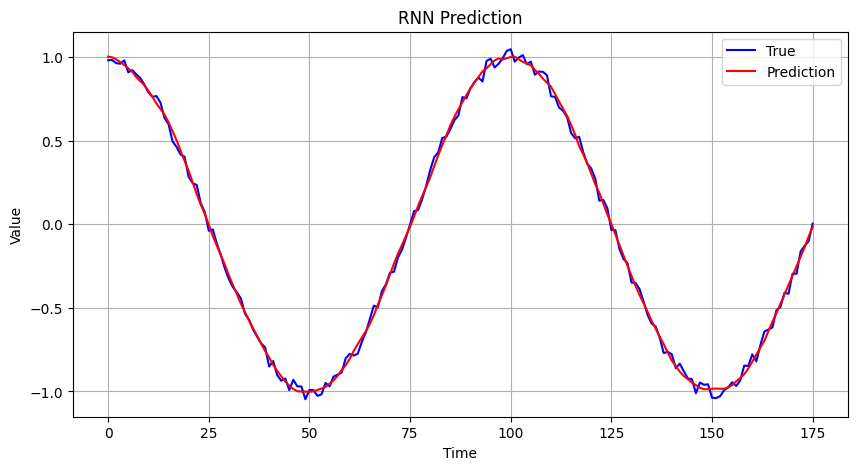
\includegraphics[width=0.8\linewidth]{images/rnn_sin_prediction.png}
  \caption{実装した RNN による sin 波の生成。
           \TODO{NumPy 実装での最新の図（Python/RNN/prediction.png）に差し替える}}
  \label{fig:sin_pred}
\end{figure}

なお、パラメータ更新に最も基本的な勾配降下法を用いた場合、
次の 1 点の予測（損失の低下）自体は達成できたが、
予測値を入力に戻して波形を生成させると形が崩れてしまった。
Adam を用いることでこの問題は解消した。
\TODO{この比較結果（表）を載せる。README.md に測定値がある}

\section{Hodgkin-Huxley モデルのシミュレーション}

\TODO{Algorithm \ref{alg:iext} で生成した外部電流と、それに対する
      HH モデルの応答（$V, m, h, n$）の図を載せる。
      先行研究の図 4.1 に相当するもの}

\section{学習結果}

\TODO{学習曲線（訓練損失・検証損失）と、最終的な損失の値を載せる}

\section{代理モデルの評価}

\TODO{\ref{sec:metrics}節の各指標について結果を載せる。
      (1) 波形の比較図と RMSE・MAE
      (2) スパイク特徴量の比較表
      (3) 定常電流振幅の掃引に対するスパイク数、ramp 電流に対する閾値、sin 波応答
      (4) 計算コストの比較表}

\section{考察}

\TODO{以下の観点で書く。
      ・RNN が HH モデルの膜電位応答をどこまで再現できたか
      ・SINDy による先行研究\cite{munechika2025}との比較。
        SINDy は微分方程式の形で解釈可能なモデルが得られる一方、
        時間計算量が増加した。RNN は解釈性に劣るが行列演算のみで構成されるため
        GPU による並列化に向く、という対比ができるはず
      ・自己回帰による誤差累積の影響
      ・学習データに含まれない入力に対する外挿性能の限界
      ・Multi-Compartment モデルへ拡張した場合に期待される計算コスト削減量の見積もり}

% ==================================================================
\chapter{まとめ}
% ==================================================================

\TODO{以下の流れで書く。
      ・本研究は RNN を用いてニューロンモデルの代理モデルを構築した
      ・RNN は PyTorch を使わず NumPy のみで実装し、BPTT が正しいことを数値微分で確認した
      ・（結果のまとめ）
      ・今後は Multi-Compartment モデルに対する代理モデルの構築を行う}

% ==================================================================
\chapter*{謝辞}
\addcontentsline{toc}{chapter}{謝辞}
% ==================================================================

本研究を進めるにあたり、多大なるご指導とご助言を賜りました小林泰良助教に
深く感謝申し上げます。
\TODO{使用したライブラリ（NumPy, Matplotlib など）への謝辞、
      先行研究の実装を参考にさせていただいた点への謝辞を書く}

% ==================================================================
% 参考文献
% ==================================================================
\begin{thebibliography}{99}

\bibitem{yamazaki2021}
山﨑 匡, 五十嵐 潤.
\newblock はじめての神経回路シミュレーション: 1 ニューロンからヒト全脳モデルまで.
\newblock 森北出版株式会社, 2021, pp.~56--61.

\bibitem{kandel2022}
Eric R. Kandel et al.
\newblock カンデル神経科学. 第 2 版.
\newblock メディカル・サイエンス・インターナショナル, 2022, p.~57.

\bibitem{gidon2020}
Albert Gidon et al.
\newblock Dendritic Action Potentials and Computation in Human Layer 2/3 Cortical Neurons.
\newblock \textit{Science}, Jan. 2020.
\newblock doi: 10.1126/science.aax6239.

\bibitem{branco2010}
Tiago Branco, Beverley A. Clark, Michael H\"ausser.
\newblock Dendritic Discrimination of Temporal Input Sequences in Cortical Neurons.
\newblock \textit{Science}, 329.5999 (Sept. 2010), p.~1671.
\newblock doi: 10.1126/science.1189664.

\bibitem{kobayashi2024}
Kobayashi Taira, Tamura Akira, Rin Kuriyama.
\newblock Development of a lightweight and customizable biophysical neuron simulator. 2024.
\newblock \url{https://researchmap.jp/tairakobayashi/presentations/48836360}

\bibitem{hodgkin1952}
A. L. Hodgkin, A. F. Huxley.
\newblock A Quantitative Description of Membrane Current and Its Application to
Conduction and Excitation in Nerve.
\newblock \textit{The Journal of Physiology}, 117.4 (Aug. 1952), pp.~500--544.
\newblock doi: 10.1113/jphysiol.1952.sp004764.

\bibitem{miyagawa2013}
宮川 博義, 井上 雅司.
\newblock ニューロンの生物物理. 第 2 版.
\newblock 丸善出版, 2013.

\bibitem{minemura2008}
峯村 吉泰.
\newblock C と Java で学ぶ数値シミュレーション入門.
\newblock 森北出版株式会社, 2008, pp.~155--157.

\bibitem{brunton2015}
Steven L. Brunton, Joshua L. Proctor, J. Nathan Kutz.
\newblock Discovering Governing Equations from Data: Sparse Identification of
Nonlinear Dynamical Systems. Sept. 2015.
\newblock doi: 10.1073/pnas.1517384113.

\bibitem{munechika2025}
棟近 春樹.
\newblock Hodgkin-Huxley モデルの計算コスト削減を目指したサロゲートモデルの開発.
\newblock 卒業論文, 山口大学理学部物理・情報科学科, 令和 6 年度.
% \TODO{先輩の卒論の引用形式を先生に確認する。
%       また、進捗報告スライド（2026年）を引用する場合の書き方も確認が必要}

\bibitem{sugomori2019}
巣籠 悠輔.
\newblock 詳解ディープラーニング 第 2 版: TensorFlow/Keras・PyTorch による時系列データ処理.
\newblock マイナビ出版, 2019.
% 第 5 章（pp.~255--277）がリカレントニューラルネットワーク

\bibitem{elman1990}
Jeffrey L. Elman.
\newblock Finding Structure in Time.
\newblock \textit{Cognitive Science}, 14.2 (1990), pp.~179--211.
\newblock doi: 10.1207/s15516709cog1402\_1.

\bibitem{werbos1990}
Paul J. Werbos.
\newblock Backpropagation Through Time: What It Does and How to Do It.
\newblock \textit{Proceedings of the IEEE}, 78.10 (Oct. 1990), pp.~1550--1560.
\newblock doi: 10.1109/5.58337.

\bibitem{saxe2014}
Andrew M. Saxe, James L. McClelland, Surya Ganguli.
\newblock Exact Solutions to the Nonlinear Dynamics of Learning in Deep Linear
Neural Networks. 2014.
\newblock arXiv: 1312.6120.

\bibitem{kingma2015}
Diederik P. Kingma, Jimmy Ba.
\newblock Adam: A Method for Stochastic Optimization. 2015.
\newblock arXiv: 1412.6980.

\bibitem{chen2019}
Ricky T. Q. Chen et al.
\newblock Neural Ordinary Differential Equations. Dec. 2019.
\newblock doi: 10.48550/arXiv.1806.07366.

\end{thebibliography}

% ==================================================================
\appendix
\chapter{付録}
% ==================================================================

\section{実装したコード}

\TODO{NumPy による RNN の実装（Python/RNN/simple\_rnn.py）の主要部分を載せるか、
      リポジトリの URL を記載する}

\end{document}
